%----------------------------------------------------------------------------------------
%	PACKAGES AND DOCUMENT CONFIGURATIONS
%----------------------------------------------------------------------------------------
\documentclass[article, a4paper, 11pt, oneside]{memoir}

% Margins
\usepackage[top=3cm,left=2cm,right=2cm,bottom=3cm]{geometry}

% Encondings
\usepackage[utf8]{inputenc}

% Language
\usepackage[portuguese]{babel}

% Graphics and images
\usepackage{graphicx}
	\graphicspath{{./images/}}

% Listings
\usepackage{listings}
\usepackage{amsmath}

% Color
\usepackage[dvipsnames]{xcolor}

% Tables
\usepackage{tabularx}

% Math symbols
\usepackage{amssymb}

% Paragraph Spacing
\usepackage{parskip}
\usepackage{indentfirst}
\setlength{\parskip}{0.5cm}

% Hyperreferences
\usepackage{hyperref}

% Repeated commands
\usepackage{expl3}
\ExplSyntaxOn
\cs_new_eq:NN \Repeat \prg_replicate:nn
\ExplSyntaxOff

% Header and Footer Things
\usepackage{wallpaper}
\usepackage{fancyhdr}

% Following code to edit the pagestyle
\pagestyle{fancy}
\fancyhf{}
\rhead{RCOM}
\lhead{\leftmark}
\rfoot{Página \thepage}

% Commands
\usepackage{xargs}

%% Linked Email
\newcommand{\email}[1]{
{\texttt{\href{mailto:#1}{#1}} }
}

%----------------------------------------------------------------------------------------
%	DOCUMENT INFORMATION
%----------------------------------------------------------------------------------------
% Title
\title{\Huge \texttt{Rede de Computadores} }
% Authors
\author{
\LARGE \textbf{Turma Grupo}\\\\
\begin{tabular}{l r}
	  Diogo Samuel Gonçalves Fernandes	& \email{up201806250@fe.up.pt}\\
	 Paulo Jorge Salgado Marinho Ribeiro  & \email{up201806505@fe.up.pt}\\
\end{tabular}
}

% Date for the report
\date{\today}

% Table of Contents
\addto\captionsportuguese{\renewcommand*\contentsname{Índice}}

%----------------------------------------------------------------------------------------
%	DOCUMENT
%----------------------------------------------------------------------------------------
\begin{document}
%----------------------------------------------------------------------------------------
%	Front Page
%----------------------------------------------------------------------------------------
% Title Author and Date
\maketitle

% More information for front page
\begin{center}
\textbf{Projeto RCOM - 2019/20 - MIEIC}
\Repeat{2}{\linebreak}
\begin{tabular}{l r}
	\textbf{Professor}: 
	\begin{tabular}{l r}
		Rui Campos & \email{rcampos@fe.up.pt}	\\
	\end{tabular}
\end{tabular}
\Repeat{4}{\linebreak}

\end{center}

\newpage
%----------------------------------------------------------------------------------------
%	CHAPTER 1 - Descrição do Problema
%----------------------------------------------------------------------------------------
\chapter[Introdução][Introdução]{Introdução} \label{\thechapter}

Tendo como principal objetivo a implementação de um protocolo de transferência de dados recorrendo a uma porta série, 
este trabalho deve resultar num programa capaz de resistir a fenómenos como a interrupção da porta série ou a receção de informação corrompida,
provocada pela indução de "ruído" na porta série. Este relatório procura explicar toda a teoria envolvida neste primeiro trabalho, de forma bem estruturada, 
nos seguintes tópicos:
\begin{itemize}
	\item Arquitetura - Descrição dos blocos funcionais e interfaces
	\item Estrutura do código - Explicação das APIs, enumeração das principais estruturas de dados utilizadas, das funções de maior importância e relação com a arquitetura
	\item Casos de Uso Principais - Identificação dos casos de uso mais importantes, e demonstração sequencial das chamadas às funções.
	\item Protocolo de ligação lógica - Identificação dos principais aspetos funcionais da camada de Ligação de Dados, descrição da estratégia de implementação destes aspetos, com o apoio de extratos de código.
	\item Protocolo de aplicação - Identificação dos principais aspetos funcionais da camada da Aplicação, descrição da estratégia de implementação destes aspetos, com o apoio de extratos de código.
	\item Validação - Descrição dos testes efetuados com apresentação quantificada dos resultados.
	\item Eficiência do protocolo de ligação de dados - Caracterização estatística da eficiência do protocolo, feita com recurso a medidas sobre o código desenvolvido.
	\item Conclusões - Síntese da informação apresentada nas secções anteriores, e reflexão sobre os objetivos de aprendizagem alcançados.
\end{itemize}

%----------------------------------------------------------------------------------------
%	CHAPTER 2 - Arquitetura
%----------------------------------------------------------------------------------------
\chapter[Arquitetura][Arquitetura]{Arquitetura} \label{\thechapter}

O programa desenvolvido desdobra-se em duas camadas bem definidas: 

\begin{itemize}
	\item A camada de Ligação de Dados (Link Layer) 
	\item A camada da Aplicação (Application Layer)
\end{itemize} 

A primeira, como é responsável pelo estabelecimento da ligação, torna o protocolo sólido, garantindo a sua consistência. 
Por este motivo, é considerada a camada de mais baixo nível do programa, sendo que trata da abertura da porta série, 
da transmissão de informação (escrita e leitura), e do seu posterior fecho. 
É também da sua responsabilidade testar se a informação foi escrita/recebida corretamente, através de byte stuffing, e de testes de erros como os BCC,
que serão aqui detalhados mais tarde.

Por outro lado, a camada da Aplicação é apenas responsável pelo envio e receção da informação dos ficheiros, pelo que é de um nível superior à camada de ligação de dados.
Assim, esta camada chama as funções da camada da ligação de dados, para envio/receção da informação de dados, 
mantendo-se, no entanto, completamente independente desta, uma vez que desconhece os seus métodos de atuar.

%----------------------------------------------------------------------------------------
%	CHAPTER 3 - Estrutura do código
%----------------------------------------------------------------------------------------
\chapter[Estrutura do código][Estrutura do código]{Estrutura do código} \label{\thechapter}

Esta independência entre camadas está também explícita na sua implementação, uma vez que o código relativo à camada de ligação de dados se encontra desenvolvido nos ficheiros “llfunctions.h” e “llfunctions.c”, enquanto que o código relativo à camada da Aplicação encontra-se nos ficheiros “writenoncanonical.c” (parte do Emissor) e “noncanonical.c” (parte do Recetor). Os ficheiros “messages.h” e “messages.c” contêm funções auxiliares usadas pelas principais funções, responsáveis pelo envio/receção de tramas e pelo cálculo do BCC2. 
Já os ficheiros “statemachines.h” e “statemachines.c” contêm o código que simula as máquinas de estados necessárias para a receção.
No ficheiro “constdefines.h” estão definidas todas as estruturas de dados utilizadas, e definidas as principais macros usadas, que enumeramos de seguida.

\section{Estruturas de Dados}
Recorremos à struct applicationLayer para armazenar a informação relativa à camada da aplicação, nomeadamente o nome da porta série a utilizar, o seu descritor de ficheiro, e um inteiro que indica se o programa está a fazer o papel de Emissor ou Recetor.

\begin{lstlisting}
struct applicationLayer {
	char port[20]; // Dispositivo /dev/ttySx, x = 0, 1
	int status; // TRANSMITTER ou RECEIVER
};
\end{lstlisting}

Recorremos também a uma enum, currentstate, que é usada pelas máquinas de estados para identificar o seu estado atual, na receção das várias tramas.
enum currentstate {start, flagrcv, arcv, crcv, bccok, datarcv, bcc2ok, stop, finished};

Funções mais importantes:
\begin{itemize}
	\item int llopen(struct applicationLayer application);
	\item int llwrite(int fd, unsigned char buffer, int length);
	\item int llread(int fd, unsigned char* buffer);
	\item int llclose(struct applicationLayer *application);
\end{itemize}

\section{Macros mais importantes}
Para além das macros referentes aos bytes especiais que compõem as diversas tramas, destacamos as seguintes:

\begin{itemize}
	\item BAUDRATE: usado na struct termios, durante o llopen(), que indica a capacidade da ligação.
	\item RECEIVER a 0, e TRANSMITTER a 1: para efeitos de distinção do papel da aplicação.
	\item TIMEOUT: que indica o tempo, em segundos, que o Emissor deve esperar resposta do Recetor, antes de reenviar a trama.
	\item MAX\textunderscore SIZE: indica o tamanho máximo, em bytes, de informação do ficheiro que cabe num pacote da aplicação.
\end{itemize}
Para melhor compreensão das macros, e da estrutura das tramas, detalhamos esse ficheiro, com explicações mais profundas.

%----------------------------------------------------------------------------------------
%	CHAPTER 4 - Casos de uso principais
%----------------------------------------------------------------------------------------
\chapter[Casos de uso principais][Casos de uso principais]{Casos de uso principais} \label{\thechapter}

\section{Makefile}
O Makefile por nós criado efetua a compilação do programa, resultando em dois executáveis diferentes, um para o Emissor (writenoncanonical) 
e outro para o Recetor (noncanonical).

\section{Emissor}
O executável relativo ao Emissor exige 2 argumentos: o nome da porta série (por exemplo /dev/ttyS1), e o nome do ficheiro que vai ser transmitido (exemplo: pinguim.gif)
A sequência de chamadas efetuada por este executável é a seguinte:
\begin{itemize}
	\item llopen: Configura a ligação entre os dois computadores, abrindo a porta série em modo de escrita e leitura. Esta configuração decorre de uma troca de tramas, a trama SET enviada pelo Emissor e a trama UA enviada pelo Recetor. Apesar de a função ser comum aos dois programas, há nela uma distinção das ações conforme o parâmetro status da struct referida no tópico anterior, recebida como parâmetro.
	\item Leitura do ficheiro e armazenamento da sua informação num array de unsigned chars.
	\item Criação do pacote de controlo Start, seguido do seu envio, já recorrendo à função llwrite().
	\item Criação dos pacotes de Informação, que resulta de uma divisão do array referido no segundo passo, e o seu respetivo envio, recorrendo também a llwrite().
	\item Criação do pacote de controlo End, seguido do seu envio, recorrendo à função llwrite().
	\item llclose(): Encerramento da ligação entre os dois computadores, através de uma troca de tramas. Neste caso, o Emissor receberá uma trama DISC, enviando como resposta outra trama DISC, e para terminar receberá uma trama UA.
\end{itemize}

\section{Recetor}
O executavel relativo ao Recetor exige tambem 2 argumentos: o nome da porta serie (por exemplo /dev/ttyS0), e o nome do ficheiro que vai ser transmitido (exemplo pinguim.gif)
 
\begin{itemize}
 	\item llopen: Configura a ligação entre os dois computadores, abrindo a porta série em modo de escrita e leitura. Esta configuração decorre de uma troca de tramas, a trama SET enviada pelo Emissor e a trama UA enviada pelo Recetor. Apesar de a função ser comum aos dois programas, há nela uma distinção das ações conforme o parâmetro status da struct referida no tópico anterior, recebida como parâmetro.
 	\item Receção do pacote de controlo Start, recorrendo à função llread().
 	\item Processamento do pacote de controlo Start recebido, de modo a receber corretamente o nome e o tamanho do ficheiro que vai ser copiado, para efeitos de apenas informar o utilizador destes dados.
 	\item Receção dos pacotes de Informação, recorrendo à função llread(). A cada pacote lido, a sua informação é processada (de modo a ficar apenas com os bytes de informação do ficheiro), e esta informação é logo de seguida escrita para o novo ficheiro, criado imediatamente antes desta receção.
 	\item Quando recebe o pacote de controlo End, o loop de receção de tramas termina.
 	\item llclose(): Encerramento da ligação entre os dois computadores, através de uma troca de tramas. Neste caso, o Recetor enviará uma trama DISC, recebendo como resposta outra trama DISC, e para terminar enviará uma trama UA.
\end{itemize}

%----------------------------------------------------------------------------------------
%	CHAPTER 5 - Protocolo de ligação lógica
%----------------------------------------------------------------------------------------
\chapter[Protocolo de ligação lógica][Protocolo de ligação lógica]{Protocolo de ligação lógica} \label{\thechapter}

\section{Principais aspetos funcionais}
\begin{itemize}
 \item Estabelecimento da ligação entre os dois computadores, com abertura da porta série
 \item Reenvio de tramas por parte do emissor, na falta de resposta.
 \item Envio e Receção de informação entre os dois computadores
 \item Byte stuffing e destuffing, de modo a evitar uma má interpretação dos bytes recebidos
 \item Coordenação entre ambos os processos relativamente às tramas a enviar/receber
 \item Controlo de Erros, isto é, deteção de informação corrompida
 \item Confirmação/Rejeição de tramas, por parte do Recetor
 \item Terminação da ligação entre os dois computadores, com fecho da porta série
\end{itemize}

\section{Estratégia de implementação}

\subsection{Estabelecimento da ligação entre os dois computadores, com abertura da porta série}
O estabelecimento da ligação lógica é realizado na função llopen() do ficheiro “llfunctions.c”, na qual é efetuada a abertura da porta série, em modo de escrita e leitura. Logo após isto, é realizada uma troca de tramas entre o Emissor e o Recetor, que confirma que a ligação foi estabelecida. Segue-se o seu procedimento:
\begin{itemize}
	\item Envio de uma trama SET pelo Emissor.
\item Receção da trama SET pelo Recetor
\item Envio da trama UA pelo Recetor, como resposta
\item Receção da trama UA pelo Emissor. No caso de o Emissor não receber resposta após TIMEOUT segundos (por motivos de interrupção da porta série, por exemplo), este reenvia a trama SET. Este procedimento é repetido TRIES vezes. Se chegar ao fim deste número de vezes sem ter recebido resposta, o programa é encerrado, indicando que a função llopen() falhou. A implementação deste TIMEOUT é descrita no próximo tópico.
\end{itemize}

\subsection{Reenvio de tramas por parte do emissor, na falta de resposta}
Neste programa, recorremos ao reenvio de tramas quando o emissor espera mais do que 
TIMEOUT segundos por uma resposta do recetor. 
A forma mais simples que encontramos de implementar 
este controlo foi alterando os valores de VMIN e VTIME. 
Alterando o valor de VMIN para 0, a função read() não ficará bloqueada à espera de 
qualquer byte, e mudando o valor de VTIME para TIMEOUT * 10 (VTIME pede unidades de 0.1 segundos) 
plica que a função read() esperará esse número de segundos, e se não receber nada durante 
esse período retorna 0. Assim, testando o valor de retorno desta função poderemos saber 
o resultado desta, pelo que, quando este for zero, o emissor deve reenviar a trama.

\subsection{Envio e Receção de informação entre os dois computadores}
O envio e receção de informação é da responsabilidade das funções llwrite() e llread(), 
que escrevem e leem uma única trama, respetivamente. 
Segue-se uma breve explicação da estrutura de cada uma destas funções:

\subsection{llwrite()}
\begin{itemize}
	\item A função começa por calcular o BCC2 com os bytes de informação recebidos como parâmetro, que fará parte da estrutura da trama.
	\item De seguida, é efetuado o byte stuffing, explicado no quarto tópico deste capítulo, tanto nos bytes de informação como no BCC2.
	\item  Após isto, é composta a trama que vai ser enviada (armazenada em buffer), começando por adicionar os primeiros bytes especiais (FLAG, A, C, BCC1), só depois os bytes de informação recebidos, e por fim o BCC2 e a última FLAG.
	\item Com a trama já composta, esta é enviada para a porta série, e é de seguida esperada uma resposta do recetor (RR/REJ), que envolve todo o procedimento de reenvio de tramas, detalhado anteriormente.
	\item Por fim, é alterado o valor do número de sequência, no caso de a resposta do recetor ser positiva (RR) e com um número de sequência diferente do atual, o que significa que o Recetor pediu uma nova trama.
\end{itemize}

\subsection{llread()}
\begin{itemize}
  	\item A função começa por receber a trama, que é processada byte a byte, recorrendo a uma máquina de estados implementada no ficheiro “statemachines.c”, nomeadamente a função processDATA(), que é uma máquina de estados específica às tramas de informação.
  	\item Uma vez que a trama recebida se trata de uma mensagem com byte stuffing, é necessário fazer o processo inverso, byte destuffing, de modo a enviar a informação correta para o novo ficheiro. Para isto, inicia-se a construção da trama destuffed na variável “buffer”, adicionando primeiro os bytes especiais (FLAG, A, C, BCC1).
  	\item Segue-se a verificação do BCC1, comparando o valor recebido com um novo valor calculado conforme o número de sequência atual. Se este valor não coincidir, a função retorna um valor negativo, que é detetado no loop de envio dos pacotes da aplicação no ficheiro “noncanonical.c”, de forma a ignorar a trama recebida.
  	\item Após isto, continua-se a preencher a variável buffer com os bytes de informação, realizando o byte destuffing.
  	\item Depois, é efetuada a verificação do BCC2, comparando-se o valor recebido com um novo cálculo deste parâmetro, usando os bytes de informação recebidos (já destuffed). No caso de estes valores não coincidirem, é enviada uma trama REJ para o emissor, que reenviará a trama. É retornado um valor negativo para que a trama recebida seja ignorada.
  	\item Por último, se o valor do número de sequência recebido for igual ao atual, isto é, se foi recebida a trama que o recetor esperava, o valor de NS é alterado, que é o equivalente a pedir a próxima trama, uma vez que é enviada uma trama RR com os campos C e BCC1 afetados com esse valor.

\end{itemize}

\subsection{Byte stuffing e destuffing, de modo a evitar uma má interpretação dos bytes recebidos}
O byte stuffing e destuffing baseia-se em simples verificações, realizadas byte a byte sobre os bytes de informação recebidos (e BCC2 também), 
que os compara aos bytes especiais, nomeadamente a FLAG (0x7e) e o ESC (0x7d). 
No caso do byte stuffing, estes bytes são transformados numa sequência de 2 bytes: 0x7d 0x5e para o primeiro e 0x7d e 0x5d para o segundo. 
No byte destuffing, é efetuado o processo inverso.
Desta forma, no caso de algum dos bytes de informação ou o BCC2 coincidir com estes bytes especiais, nunca serão confundidos com os bytes especiais da trama, 
pelo que a informação é transmitida corretamente.

\subsection{Coordenação entre ambos os processos relativamente às tramas a enviar/receber}
A coordenação entre o emissor e o recetor é feita recorrendo ao “número de sequência”,
 que pode tomar o valor 0 ou 1, e que vem implícito no campo C das tramas. 
 O número de sequência de ambos os processos começa a 0. 
 As respostas do recetor (RR/REJ) indicam o recetor se deve reenviar a trama atual,
  ou se deve enviar uma nova trama. É necessário reenvio quando o valor do número de sequência 
  recebido pelo emissor é igual ao seu atual, isto é, o recetor pediu o reenvio da trama, 
  devido a erros na informação. Por outro lado, quando o valor do número de sequência recebido 
  pelo emissor é diferente do seu atual, este deve passar para a próxima trama, 
  uma vez que esta foi requisitada pelo recetor. Esta alternância entre os dois 
  valores possíveis do número de sequência permite esta coordenação entre os dois processos.

\subsection{Controlo de Erros, isto é, deteção de informação corrompida}
O controlo de erros é feito a dois níveis: BCC1, que diz respeito à numeração da trama recebida,
 e BCC2, que está relacionado com os bytes de informação da trama. 
 O primeiro é calculado realizando o XOR entre os campos A e C da trama, 
 e comparado com o valor do BCC1 recebido na trama. Em caso de não coincidirem, 
 indica um erro na numeração das tramas, e o recetor ignora a trama. Já o BCC2 é 
 calculado realizando o XOR entre todos os bytes de informação da trama, e 
 comparado com o valor do BCC2 recebido na trama. No caso de não coincidirem, 
 é porque a informação está corrompida (devido ao chamado “ruído”), 
 pelo que é enviada uma trama REJ, que indica ao emissor que deve reenviar a trama.

\subsection{Confirmação/Rejeição de tramas, por parte do Recetor}
A confirmação da trama ocorre quando não há qualquer erro na trama recebida e o número de sequência recebido coincide com o seu atual. 
Nesse caso, ele simplesmente altera o valor do número de sequência, o que significa que pede uma nova trama.
A rejeição da trama ocorre quando há algum erro na trama, seja ele no BCC1 ou no BCC2, ou então quando o número de sequência recebido não coincide com o atual do recetor.
 No caso de erros no BCC1, a trama é simplesmente ignorada, e o recetor espera por um reenvia desta. 
 No caso de erros no BCC2, é enviada uma trama REJ, que pede um reenvio da trama ao emissor. 
 Já no caso de discrepância entre os números de sequências, é enviada uma trama RR com o número de sequência atual, para que o emissor saiba que deve reenviar a trama.
 \subsection{Terminação da ligação entre os dois computadores, com fecho da porta série}
A terminação da ligação lógica é realizado na função llclose() do ficheiro “llfunctions.c”. 
Baseia-se numa troca de tramas entre o Emissor e o Recetor, que confirma a terminação da ligação. 
Segue-se o seu procedimento:
\begin{itemize}
	\item Envio de uma trama DISC pelo Emissor.
	\item Receção da trama DISC pelo Recetor
	\item Envio de uma trama DISC pelo Recetor
	\item Receção da trama DISC pelo Emissor
	\item Envio de uma trama UA pelo Emissor
	\item Receção da trama UA pelo Recetor
\end{itemize}


\newpage
%----------------------------------------------------------------------------------------
%	CHAPTER 6 - Protocolo de aplicação
%----------------------------------------------------------------------------------------
\chapter[Protocolo de aplicação][Protocolo de aplicação]{Protocolo de aplicação} \label{\thechapter}
  
\section{Principais aspetos funcionais}
\begin{itemize}
  \item Leitura do ficheiro a enviar, por parte do emissor, e criação/escrita de um ficheiro destino por parte do recetor
  \item Envio e Receção dos pacotes de controlo START e END
  \item Divisão da informação do ficheiro conforme o valor de MAX\textunderscore SIZE, e construção dos pacotes de dados, respeitando a sua estrutura
\end{itemize}

\section{Estratégia de implementação}
\subsection{Leitura do ficheiro a enviar, por parte do emissor, e criação/escrita de um ficheiro destino por parte do recetor.} 

Logo após estabelecer a ligação com o Recetor, o Emissor efetua a abertura do ficheiro a ser copiado, e lê a informação desta,
copiando-a para um array fileData, no ficheiro “writenoncanonical.c”. Armazena também o 
tamanho deste ficheiro, na variável sizeFile. Por outro lado, o Recetor, sabendo o tamanho 
do ficheiro, que veio no pacote de controlo START, abre o ficheiro destino (ou cria-o, se 
este ainda não existir), e vai escrevendo a informação recebida para este, a cada pacote recebido.

\subsection{Envio e Receção dos pacotes de controlo START e END}
O Emissor começa por criar o pacote de controlo START, que tem a seguinte estrutura:

\begin{figure}[h]
	\centering
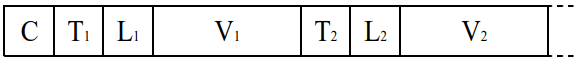
\includegraphics[scale=0.4]{trama-2.png}
\caption{\emph{Trama de controlo}}
\end{figure}


Este irá conter dois tipos de informação (dois parâmetros na forma TLV), o tamanho e o nome do ficheiro,
 e o campo C terá o valor 2 (que indica que se trata de um pacote START). 
Estas informações serão recebidas pelo Recetor, que apresentará no ecrã estes dados.
Após enviar todos os pacotes de dados, o Emissor cria o pacote de controlo END, que será igual ao START, com exceção 
 campo C, que terá o valor 3 (indicador do pacote END). 
O Recetor, recebendo este pacote, saberá que não receberá mais informação, pelo que termina o loop de receção dos
 pacotes, no ficheiro “noncanonical.c”.

\subsection{Divisão da informação do ficheiro conforme o valor de MAX\textunderscore SIZE, e construção de dados, respeitando a 
sua estrutura}

A constante MAX\textunderscore SIZE definida no ficheiro “constdefines.h” indica o número de bytes de informação do
ficheiro que cada pacote de dados pode conter, no máximo.
No ficheiro “writecanonical.c”, o emissor começa por calcular o número de pacotes que será preciso enviar, 
calculado com base no tamanho do ficheiro e no valor desta constante. De seguida, executa um ciclo for, de modo 
a executar uma iteração para cada pacote. 
Assim, em cada iteração, calcula o número de bytes de informação que o pacote conterá, que corresponde ao 
mínimo entre MAX\textunderscore SIZE e o número de bytes de informação 
restantes no ficheiro. Após isto, preenche os bytes especiais do pacote de dados (C, N, L2, L1), seguindo-se 
os bytes de informação a mandar. Do lado do Recetor, 
este não necessita de conhecer o tamanho do pacote de dados que receberá , uma vez que a camada da ligação 
lógica permite que este saiba quando um pacote termina – quando recebe a última FLAG. Segue-se um esquema 
da estrutura dos pacotes de aplicação:


%----------------------------------------------------------------------------------------
%	CHAPTER 7 - Validação
%----------------------------------------------------------------------------------------
\chapter[Validação][Validação]{Validação} \label{\thechapter}

Para validação do nosso programa, foram efetuados vários testes, aos quais resistiu. Destacam-se os seguintes:

\begin{itemize}
	\item Envio de ficheiros de diversos tamanhos
	\item Envio de um ficheiro com variacão do baudrate
	\item Envio de um ficheiro com variacao do tamanho dos pacotes max\textunderscore size
	\item Interrupção da porta série por alguns segundos, e retoma desta antes do encerramento do programa
	\item Indução de ruído na porta série, de modo a induzir erros na transmissão da informação das tramas
\end{itemize}

\begin{figure}[h]
	\centering
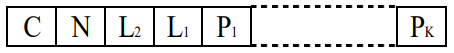
\includegraphics[scale=0.4]{trama-1.png}
\caption{\emph{Pacotes de aplicação}}
\end{figure}

%----------------------------------------------------------------------------------------
%	CHAPTER 8 - Estrutura do código
%----------------------------------------------------------------------------------------
\chapter[Eficiência do protocolo de ligação de dados][Eficiência do protocolo de ligação de dados]{Eficiência do protocolo de ligação de dados} \label{\thechapter}

Com o objetivo de avaliar a eficiência da nossa aplicação, efetuamos vários testes, com alterações a nível da capacidade
da ligação (Baudrate), do tamanho dos campos de data das tramas I (MAX\textunderscore SIZE), da percentagem de erros (FER) e dos atrasos de propagação.

\section{Variação do FER}

Pela análise do gráfico podemos concluir que, como era esperado, uma maior percentagem de erros
induzidos nas tramas I leva a uma menor eficiência do programa, devido ao facto de o tratamento destes erros ocupar grande parte do tempo de execução
(reenvio de tramas, no caso de erros no BCC2, e espera de TIMEOUT segundos por parte do emissor, no caso de erros no BCC1).

\begin{figure}[h]
	\centering
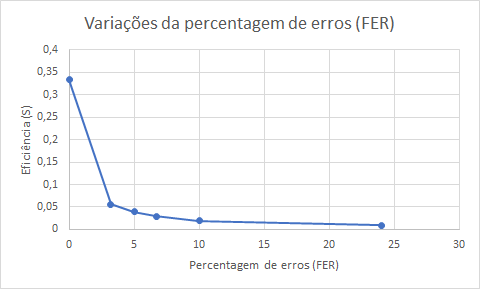
\includegraphics[scale=0.4]{fer.png}
\caption{\emph{Variação do FER}}
\end{figure}

\section{Variação do tamanho dos campos de informação das tramas I}

Analisando este gráfico, rapidamente se conclui que quando maior for o valor do MAX\textunderscore SIZE, que corresponde ao tamanho dos campos Data das tramas I,
maior será a eficiência do programa. Isto acontece porque, dado o aumento do tamanho das tramas, menor será o número de tramas enviadas, pelo que a
divisão dos pacotes será mais rápida, o que leva a um menor tempo de execução.

\begin{figure}[h]
	\centering
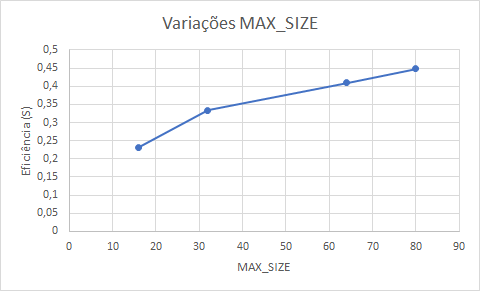
\includegraphics[scale=0.4]{maxsize.png}
\caption{\emph{Variação do max size}}
\end{figure}

\section{Variação da capacidade da ligação (Baudrate)}

Este gráfico é também de fácil análise, concluindo-se que uma maior capacidade da ligação (Baudrate) leva a uma menor eficiência do programa.
Ora, uma razão que encontramos para esta variação consiste ????

\begin{figure}[h]
	\centering
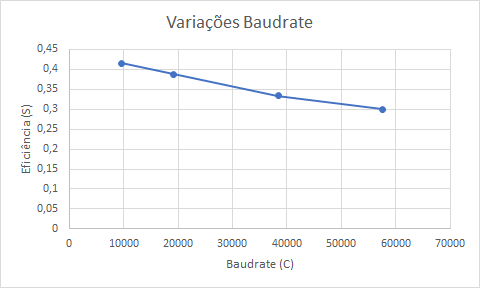
\includegraphics[scale=0.4]{baudrate.png}
\caption{\emph{Variação da baudrate}}
\end{figure}


,\section{Variação dos atrasos de propagação}
, ten
dPela análise deste gráfico conclui-se que quanto maior for o atraso de propagação,o em conta que a eficiência e a baudrate são
inversamente proporcionais, como é possível verificar na fórmula usada (S = R/C). menor será a eficiência, e este decréscimo
dá-se de forma acentuada, uma vez que a maior parte do tempo de execução resultará destes atrasos, e não do tempo útil do programa.

\begin{figure}[h]
	\centering
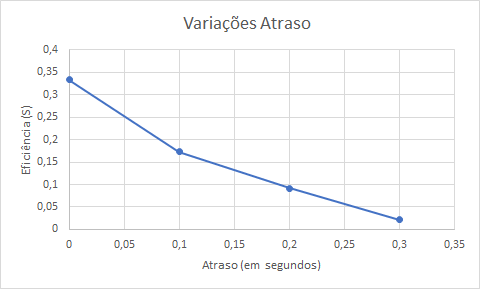
\includegraphics[scale=0.4]{atraso.png}
\caption{\emph{Variação dos atrasos de propagação}}
\end{figure}

%----------------------------------------------------------------------------------------
%	CHAPTER 9 - Conclusões
%----------------------------------------------------------------------------------------
\chapter[Conclusões][Conclusões]{Conclusões} \label{\thechapter}

A implementação do protocolo de ligação de dados que constituía o tema deste projeto deu-nos a conhecer novos conceitos, como o mecanismo Stop and Wait e tramas, 
que pudemos meter em prática durante a sua implementação. O nosso grupo conseguiu terminar todas as metas que tínhamos em mente quando iniciamos o projeto,
 tendo passado no entanto por algumas dificuldades, aquando de todos os pormenores que permitem tornar a aplicação resistente a fenómenos de erros. 
 
 Para um melhor entendimento de todos os mecanismos envolvidos no protocolo, 
 foi necessário estudar com atenção os slides acerca deste projeto, pelo que com o tempo solidificamos o 
 nosso conhecimento sobre o assunto e conseguimos resolver os problemas que encontramos.
Em suma, o projeto foi concluído com sucesso, apesar do reduzido tempo de acesso aos laboratórios, aquando das condições pandémicas que se vivem, 
e serviu para um aprofundamento 
do conhecimento teórico e prático sobre ligações de dados, e as camadas que estas envolvem.



\end{document}